\documentclass[12pt,a4paper]{article}

% ------------------------------------------------
% PAQUETES
% ------------------------------------------------

\usepackage[utf8]{inputenc}
\usepackage[T1]{fontenc}
\usepackage[spanish,es-nodecimaldot]{babel}

\usepackage{amsmath}
\usepackage{amssymb}

\usepackage{graphicx}
\usepackage{float}
\usepackage{booktabs}
\usepackage{array}

\usepackage{hyperref}

\usepackage{geometry}
\geometry{
    top=2.5cm,
    bottom=2.5cm,
    left=2.8cm,
    right=2.8cm
}

\usepackage{setspace}
\onehalfspacing

\usepackage{parskip}

\usepackage{fancyhdr}
\pagestyle{fancy}
\fancyhf{}
\rhead{Método de Monte Carlo}
\lhead{Cadenas de Markov}
\cfoot{\thepage}

% ------------------------------------------------
% INFORMACIÓN DEL DOCUMENTO
% ------------------------------------------------

\title{
    \textbf{Método de Monte Carlo aplicado a la aproximación de \(\pi\)}
}

\author{
    Henry Giovani Barrera Martínez
    Laura Victoria Torres Pinilla 
}

\date{\today}

% ------------------------------------------------
% DOCUMENTO
% ------------------------------------------------

\begin{document}

% ------------------------------------------------
% PORTADA
% ------------------------------------------------

\begin{titlepage}

    \centering

    \vspace*{2cm}

    {\Large \textbf{Universidad Nacional de Colombia}\par}

    \vspace{0.5cm}

    {\large Departamento de Matemáticas\par}

    \vspace{2cm}

    {\LARGE
    \textbf{Método de Monte Carlo aplicado a la aproximación de \(\pi\)}
    \par}

    \vspace{1.5cm}

    {\large Asignatura: Cadenas de Markov\par}

    \vspace{2cm}

    {\large
    \textbf{Estudiantes:}\\
        Henry Giovani Barrera Martínez\\
        Laura Victoria Torres Pinilla
    \par}

    \vfill

    {\large Bogotá D.C., Colombia\par}

    {\large \today\par}

\end{titlepage}

% ------------------------------------------------
% CONTENIDO
% ------------------------------------------------

\tableofcontents

\newpage

% ------------------------------------------------
% 1. INTRODUCCIÓN
% ------------------------------------------------

\section{Introducción}

El método de Monte Carlo constituye una herramienta fundamental para
resolver problemas matemáticos y estadísticos mediante procedimientos
computacionales basados en la generación de variables aleatorias.
La idea principal consiste en aproximar cantidades de interés mediante
frecuencias relativas obtenidas a partir de un número suficientemente
grande de simulaciones.

En este trabajo se estudia una aplicación geométrica del método de
Monte Carlo para aproximar el valor de la constante matemática
\(\pi\). Para ello se consideran puntos generados uniformemente en el
cuadrado

\[
\Omega=[-2,2]\times[-2,2],
\]

y se analiza la probabilidad de que un punto generado aleatoriamente
pertenezca a determinados círculos centrados en el origen.

En particular, se consideran los radios

\[
r=1,\qquad r=\sqrt{2},\qquad r=2.
\]

A partir de las probabilidades asociadas a estos conjuntos se construyen
estimadores de \(\pi\), los cuales son evaluados mediante simulaciones
con diferentes tamaños de muestra.

Finalmente, se comparan los resultados obtenidos, se analiza el
comportamiento del error y se estudia la varianza del estimador para
los diferentes radios considerados.

% ------------------------------------------------
% 2. OBJETIVOS
% ------------------------------------------------

\section{Objetivos}

\subsection{Objetivo general}

Aplicar el método de Monte Carlo para aproximar el valor de \(\pi\)
mediante la estimación de probabilidades asociadas a círculos contenidos
en un dominio rectangular.

\subsection{Objetivos específicos}

\begin{itemize}

    \item Definir el espacio de simulación y los conjuntos geométricos
    utilizados para la estimación.

    \item Estimar mediante simulación la probabilidad de que un punto
    aleatorio pertenezca al círculo de radio \(1\).

    \item Construir un estimador de \(\pi\) a partir de la probabilidad
    estimada.

    \item Comparar el comportamiento del estimador para los radios
    \(1\), \(\sqrt{2}\) y \(2\).

    \item Analizar la convergencia del estimador y el comportamiento
    del error al aumentar el número de simulaciones.

    \item Estudiar la varianza del estimador para los diferentes radios.

\end{itemize}

% ------------------------------------------------
% 3. METODOLOGÍA
% ------------------------------------------------

\section{Metodología}

\subsection{Espacio de simulación}

Se considera como espacio de simulación el cuadrado

\[
\Omega=[-2,2]\times[-2,2].
\]

Su área es

\[
|\Omega|=4\cdot4=16.
\]

Los puntos utilizados en la simulación son generados de manera
independiente y uniforme sobre este cuadrado. Es decir, para cada
simulación se generan dos variables aleatorias independientes

\[
X\sim U(-2,2),
\qquad
Y\sim U(-2,2),
\]

y se considera el punto aleatorio

\[
(X,Y).
\]

\subsection{Conjuntos circulares}

Para cada radio \(r\) se define el conjunto

\[
C_r=
\left\{
(x,y)\in\Omega:
x^2+y^2\leq r^2
\right\}.
\]

En particular, se consideran los tres valores

\[
r=1,\qquad r=\sqrt{2},\qquad r=2.
\]

El área del círculo de radio \(r\) es

\[
|C_r|=\pi r^2.
\]

Para los radios utilizados, los círculos se encuentran contenidos en el
cuadrado de simulación. Por lo tanto, la probabilidad de pertenencia
puede calcularse mediante la razón entre las áreas:

\[
P(C_r)
=
\frac{|C_r|}{|\Omega|}
=
\frac{\pi r^2}{16}.
\]

\subsection{Generación de puntos aleatorios}

Para una muestra de tamaño \(n\), se generan los puntos

\[
(X_1,Y_1),\ldots,(X_n,Y_n).
\]

Para cada punto se verifica la condición

\[
X_i^2+Y_i^2\leq r^2.
\]

Si la condición se cumple, el punto pertenece a \(C_r\).

Definimos entonces la variable indicadora

\[
I_i^{(r)}
=
\begin{cases}
1, & \text{si }X_i^2+Y_i^2\leq r^2,\\
0, & \text{en otro caso}.
\end{cases}
\]

El número de puntos que pertenecen al círculo es

\[
N_n(C_r)=
\sum_{i=1}^{n}I_i^{(r)}.
\]

La probabilidad se estima mediante la frecuencia relativa

\[
\widehat{P}_n(C_r)
=
\frac{N_n(C_r)}{n}.
\]

% ------------------------------------------------
% 4. DESARROLLO MATEMÁTICO
% ------------------------------------------------

\section{Desarrollo matemático}

\subsection{Probabilidad del conjunto \(C_1\)}

Para \(r=1\), el conjunto corresponde al círculo unitario:

\[
C_1=
\left\{
(x,y)\in\Omega:
x^2+y^2\leq1
\right\}.
\]

Su área es

\[
|C_1|=\pi.
\]

Como el área del espacio de simulación es \(16\), se obtiene

\[
P(C_1)
=
\frac{\pi}{16}.
\]

Utilizando el valor de referencia

\[
\pi\approx3.14159265,
\]

tenemos

\[
P(C_1)
\approx
\frac{3.14159265}{16}
\approx
0.19634954.
\]

\subsection{Estimación mediante Monte Carlo}

La estimación de la probabilidad se obtiene mediante

\[
\widehat{P}_n(C_1)
=
\frac{N_n(C_1)}{n}.
\]

Por la Ley de los Grandes Números,

\[
\widehat{P}_n(C_1)
\longrightarrow
P(C_1)
\]

cuando

\[
n\longrightarrow\infty.
\]

Por lo tanto, al aumentar el número de puntos simulados, la frecuencia
relativa de puntos pertenecientes al círculo debe aproximarse al valor
teórico de \(P(C_1)\).

\subsection{Estimación de \(\pi\)}

Partiendo de

\[
P(C_1)=\frac{\pi}{16},
\]

se despeja \(\pi\):

\[
\pi=16P(C_1).
\]

Por consiguiente, el estimador de Monte Carlo es

\[
\boxed{
\widehat{\pi}_n
=
16\widehat{P}_n(C_1)
}
\]

o equivalentemente,

\[
\widehat{\pi}_n
=
16\frac{N_n(C_1)}{n}.
\]

Este estimador permite aproximar \(\pi\) directamente a partir de los
puntos generados aleatoriamente.

\subsection{Generalización para los radios considerados}

Para un radio general \(r\),

\[
P(C_r)=\frac{\pi r^2}{16}.
\]

Despejando \(\pi\),

\[
\pi
=
\frac{16P(C_r)}{r^2}.
\]

Por tanto, el estimador correspondiente es

\[
\boxed{
\widehat{\pi}_n(r)
=
\frac{16}{r^2}
\widehat{P}_n(C_r)
}
\]

y se obtienen los siguientes casos particulares:

\[
r=1:
\qquad
\widehat{\pi}_n
=
16\widehat{P}_n(C_1),
\]

\[
r=\sqrt{2}:
\qquad
\widehat{\pi}_n
=
8\widehat{P}_n(C_{\sqrt{2}}),
\]

\[
r=2:
\qquad
\widehat{\pi}_n
=
4\widehat{P}_n(C_2).
\]

% ------------------------------------------------
% 5. RESULTADOS
% ------------------------------------------------

\section{Resultados}

\subsection{Aproximación de \(P(C_1)\)}

Se realizaron simulaciones utilizando tamaños de muestra

\[
n=100,\;1000,\;10000,\;100000,\;1000000.
\]

Los resultados obtenidos para el círculo unitario se presentan en la
Tabla~\ref{tab:probabilidad}.

\begin{table}[H]
\centering
\caption{Aproximación de \(P(C_1)\).}
\label{tab:probabilidad}

\begin{tabular}{rrrr}
\toprule
\(n\) & Puntos dentro & \(\widehat{P}_n(C_1)\) &
Error absoluto \\
\midrule
100 & 25 & 0.250000 & 0.053650 \\
1\,000 & 189 & 0.189000 & 0.007350 \\
10\,000 & 1\,945 & 0.194500 & 0.001850 \\
100\,000 & 19\,436 & 0.194360 & 0.001990 \\
1\,000\,000 & 196\,517 & 0.196517 & 0.000167 \\
\bottomrule
\end{tabular}

\end{table}

El valor teórico utilizado como referencia es

\[
P(C_1)\approx0.19634954.
\]

Se observa que la estimación para \(n=1\,000\,000\) es

\[
\widehat{P}_{1\,000\,000}(C_1)=0.196517,
\]

con un error absoluto de aproximadamente

\[
0.000167.
\]

\subsection{Aproximación de \(\pi\) mediante \(C_1\)}

Utilizando

\[
\widehat{\pi}_n
=
16\widehat{P}_n(C_1),
\]

se obtienen los resultados de la Tabla~\ref{tab:pi}.

\begin{table}[H]
\centering
\caption{Aproximación de \(\pi\) mediante el círculo unitario.}
\label{tab:pi}

\begin{tabular}{rrrr}
\toprule
\(n\) & \(\widehat{P}_n(C_1)\) &
\(\widehat{\pi}_n\) & Error absoluto \\
\midrule
100 & 0.250000 & 4.000000 & 0.858407 \\
1\,000 & 0.189000 & 3.024000 & 0.117593 \\
10\,000 & 0.194500 & 3.112000 & 0.029593 \\
100\,000 & 0.194360 & 3.109760 & 0.031833 \\
1\,000\,000 & 0.196517 & 3.144272 & 0.002679 \\
\bottomrule
\end{tabular}

\end{table}

El valor de referencia utilizado es

\[
\pi\approx3.14159265.
\]

Para el mayor tamaño de muestra se obtiene

\[
\widehat{\pi}_{1\,000\,000}
=
3.144272,
\]

con un error absoluto de aproximadamente

\[
0.002679.
\]

\subsection{Comparación entre los diferentes radios}

La Tabla~\ref{tab:radios} presenta las estimaciones obtenidas para los
tres radios considerados.

\begin{table}[H]
\centering
\caption{Estimación de \(\pi\) para diferentes radios.}
\label{tab:radios}

\begin{tabular}{rrrr}
\toprule
\(n\) & \(r=1\) & \(r=\sqrt{2}\) & \(r=2\) \\
\midrule
100 & 4.000000 & 3.280000 & 3.040000 \\
1\,000 & 3.024000 & 3.256000 & 3.100000 \\
10\,000 & 3.112000 & 3.151200 & 3.128000 \\
100\,000 & 3.109760 & 3.142080 & 3.138440 \\
1\,000\,000 & 3.144272 & 3.140752 & 3.142352 \\
\bottomrule
\end{tabular}

\end{table}

Para \(n=1\,000\,000\), los errores absolutos correspondientes son:

\[
\left|\widehat{\pi}(1)-\pi\right|
=
0.002679,
\]

\[
\left|\widehat{\pi}(\sqrt{2})-\pi\right|
=
0.000841,
\]

y

\[
\left|\widehat{\pi}(2)-\pi\right|
=
0.000759.
\]

Por lo tanto, en esta simulación el radio \(r=2\) produce la
aproximación más cercana al valor de \(\pi\).

% ------------------------------------------------
% 6. GRÁFICAS
% ------------------------------------------------

\section{Representación gráfica}

\subsection{Convergencia de la estimación de \(\pi\)}

La Figura~\ref{fig:convergencia} muestra el comportamiento de la
estimación de \(\pi\) a medida que aumenta el número de simulaciones.

\begin{figure}[H]
\centering
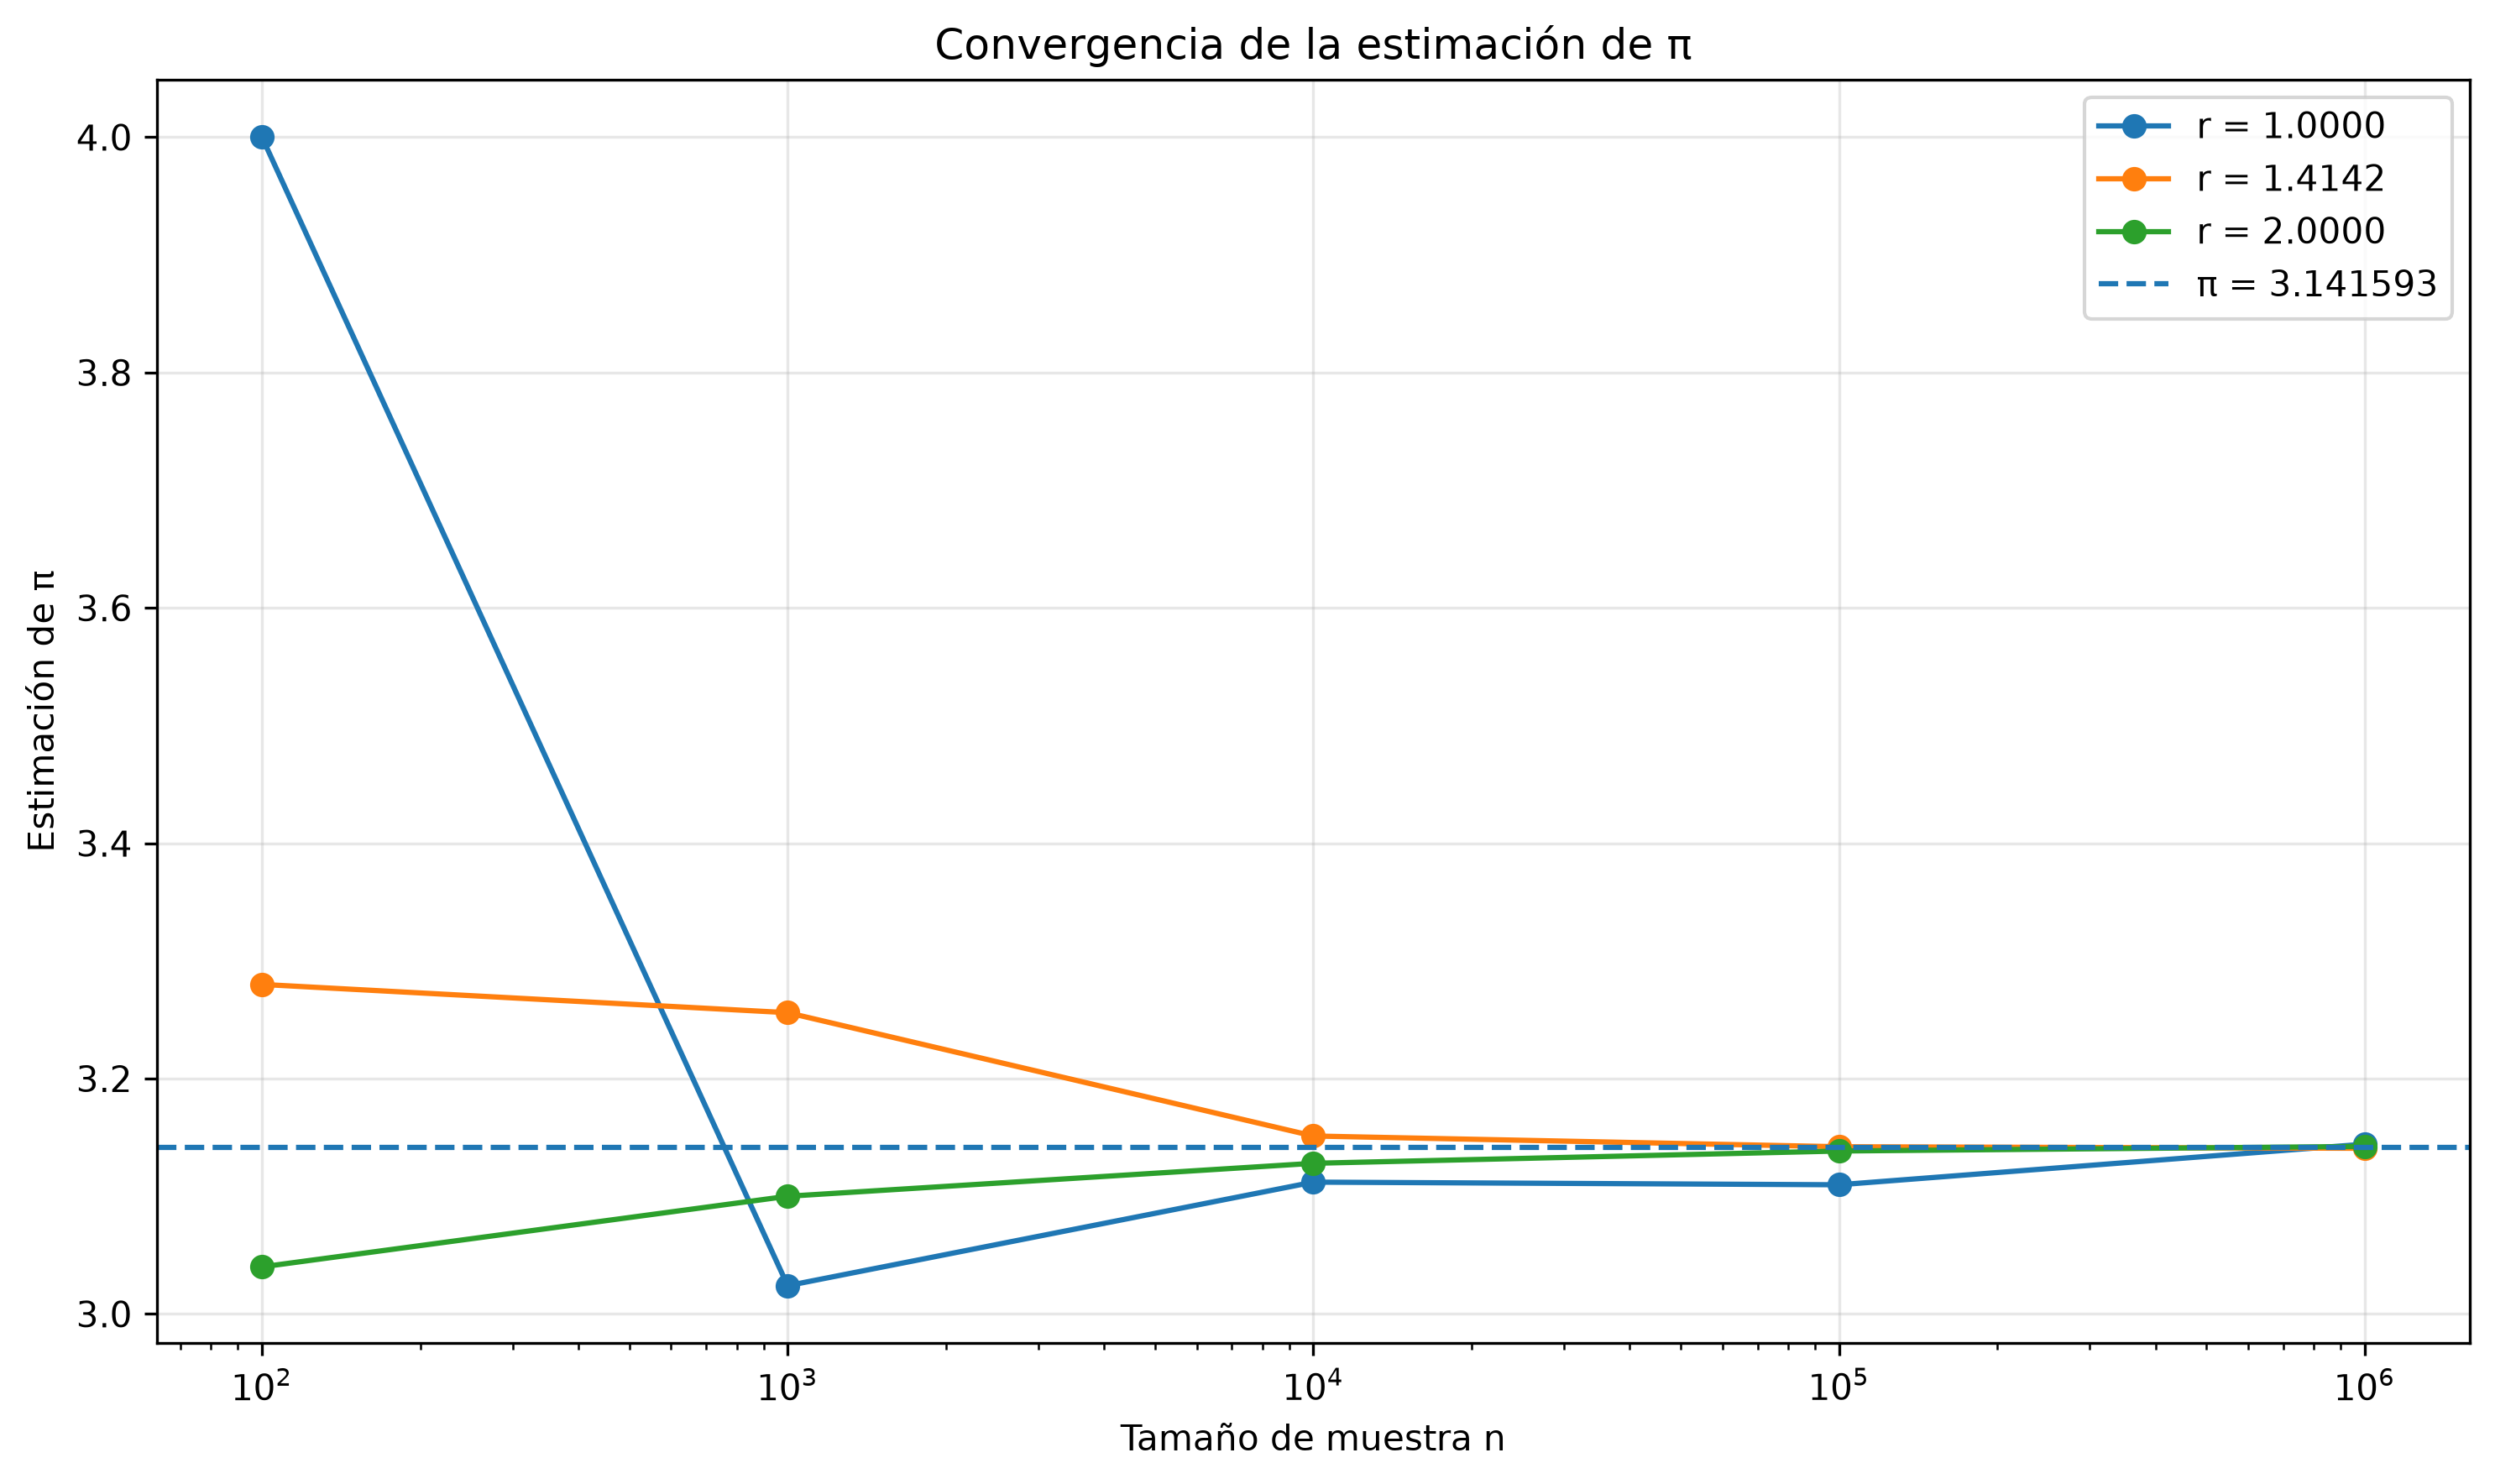
\includegraphics[width=0.85\textwidth]{../results/convergencia_pi.png}
\caption{Convergencia de la estimación de \(\pi\).}
\label{fig:convergencia}
\end{figure}

Se observa que, a medida que aumenta el tamaño de la muestra, las
estimaciones presentan una tendencia hacia el valor verdadero de
\(\pi\).

\subsection{Error absoluto}

La evolución del error absoluto se presenta en la
Figura~\ref{fig:error}.

\begin{figure}[H]
\centering
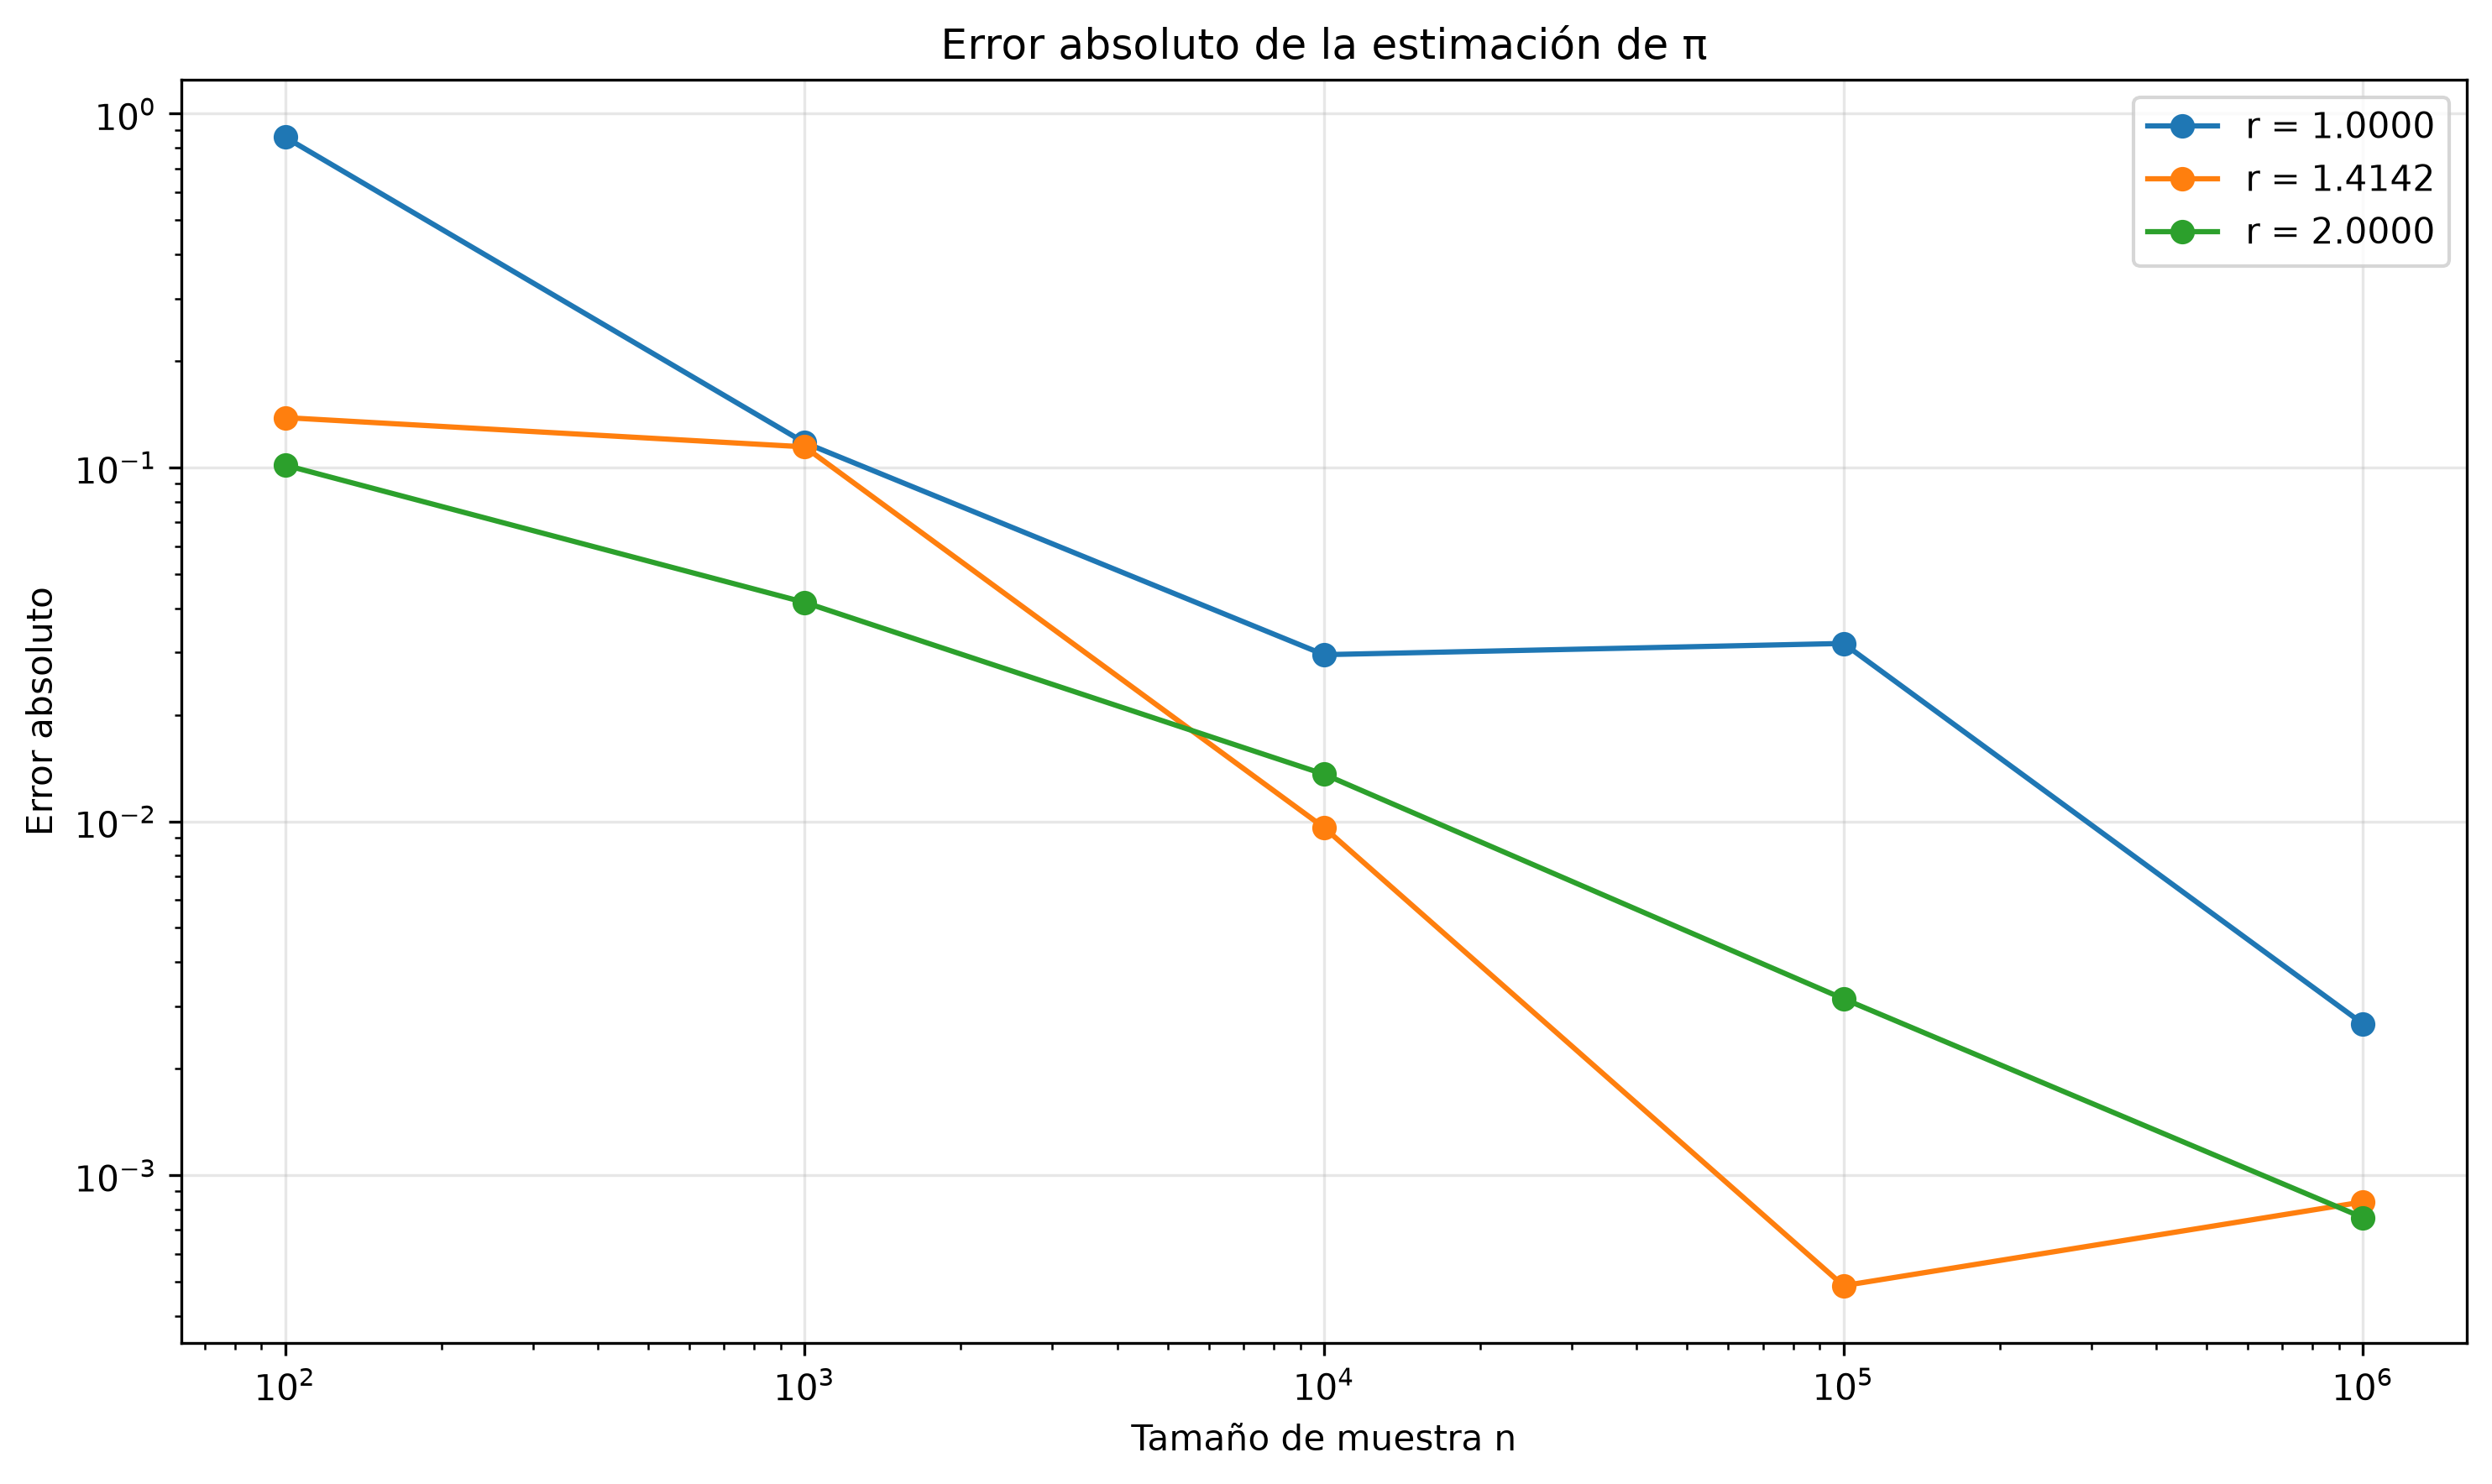
\includegraphics[width=0.85\textwidth]{../results/error_pi.png}
\caption{Error absoluto de la estimación de \(\pi\).}
\label{fig:error}
\end{figure}

El comportamiento del error presenta fluctuaciones debido a la
naturaleza aleatoria de la simulación. Por esta razón, el error no
tiene que disminuir estrictamente en cada aumento del tamaño de
muestra.

\subsection{Simulación para \(r=1\)}

\begin{figure}[H]
\centering
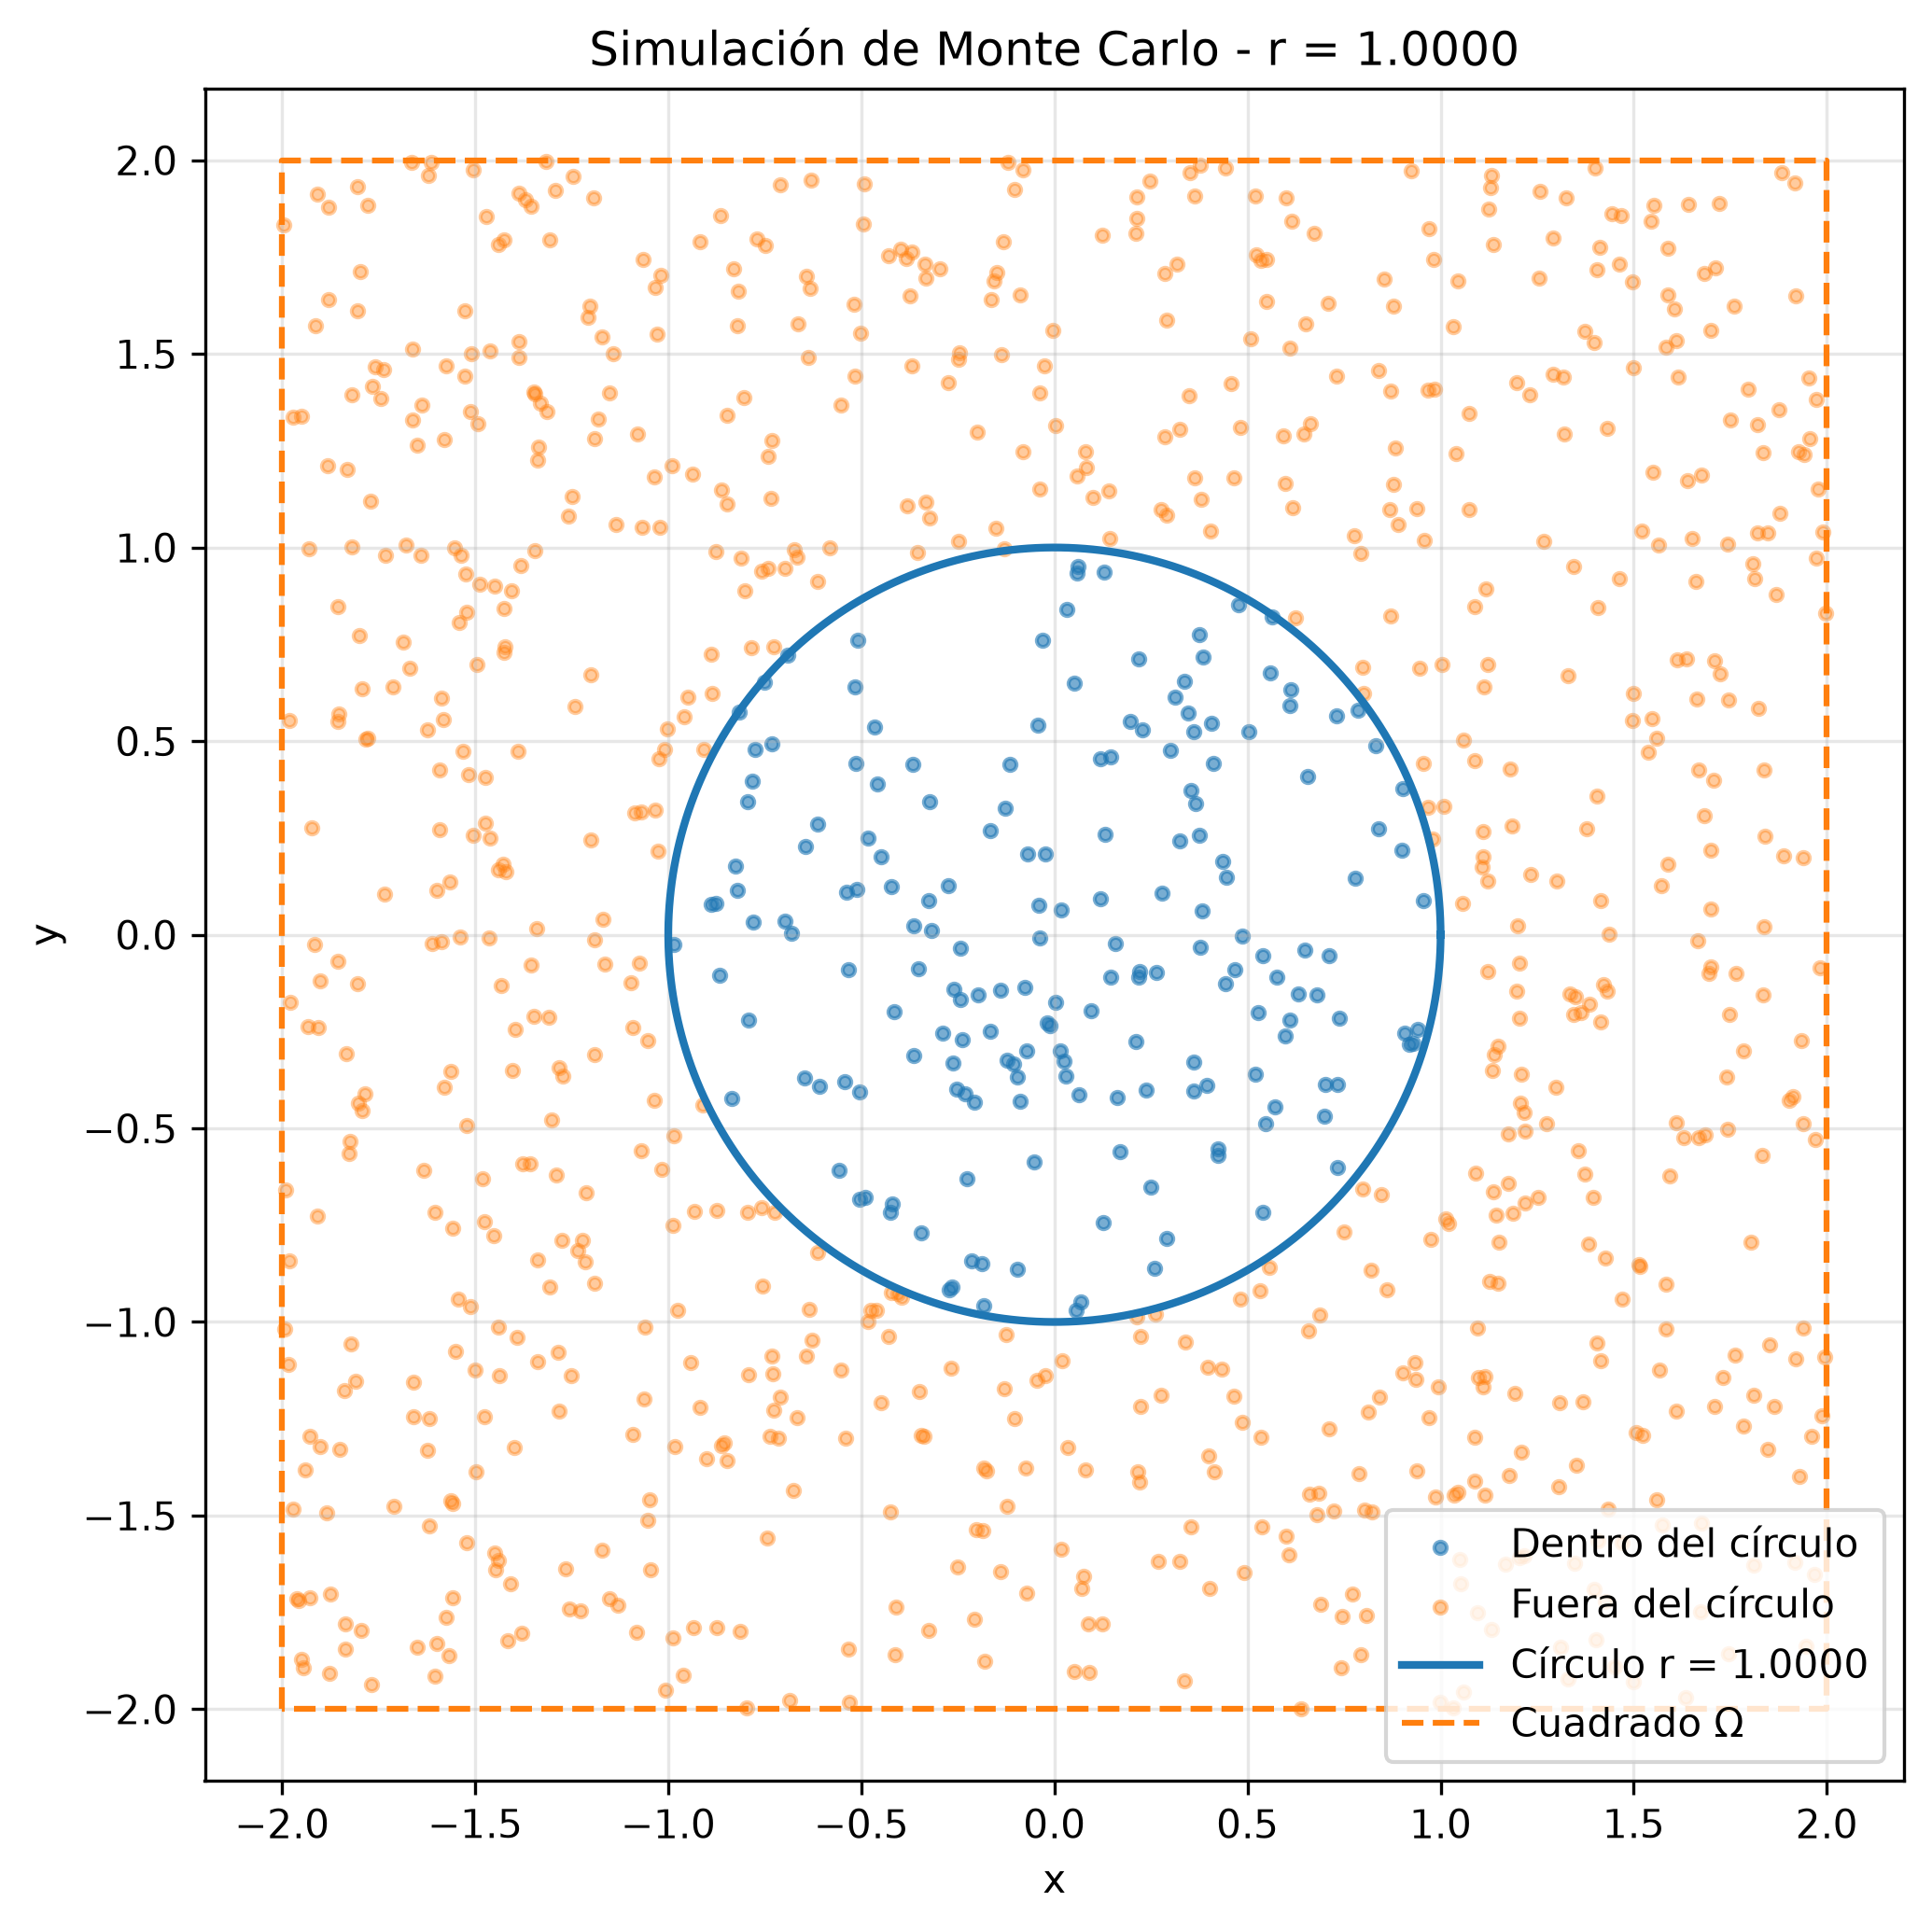
\includegraphics[width=0.75\textwidth]{../results/puntos_radio_1.png}
\caption{Puntos simulados y círculo de radio \(1\).}
\label{fig:r1}
\end{figure}

La Figura~\ref{fig:r1} muestra la distribución de los puntos generados
aleatoriamente y la región correspondiente al círculo unitario.

\subsection{Simulación para \(r=\sqrt{2}\)}

\begin{figure}[H]
\centering
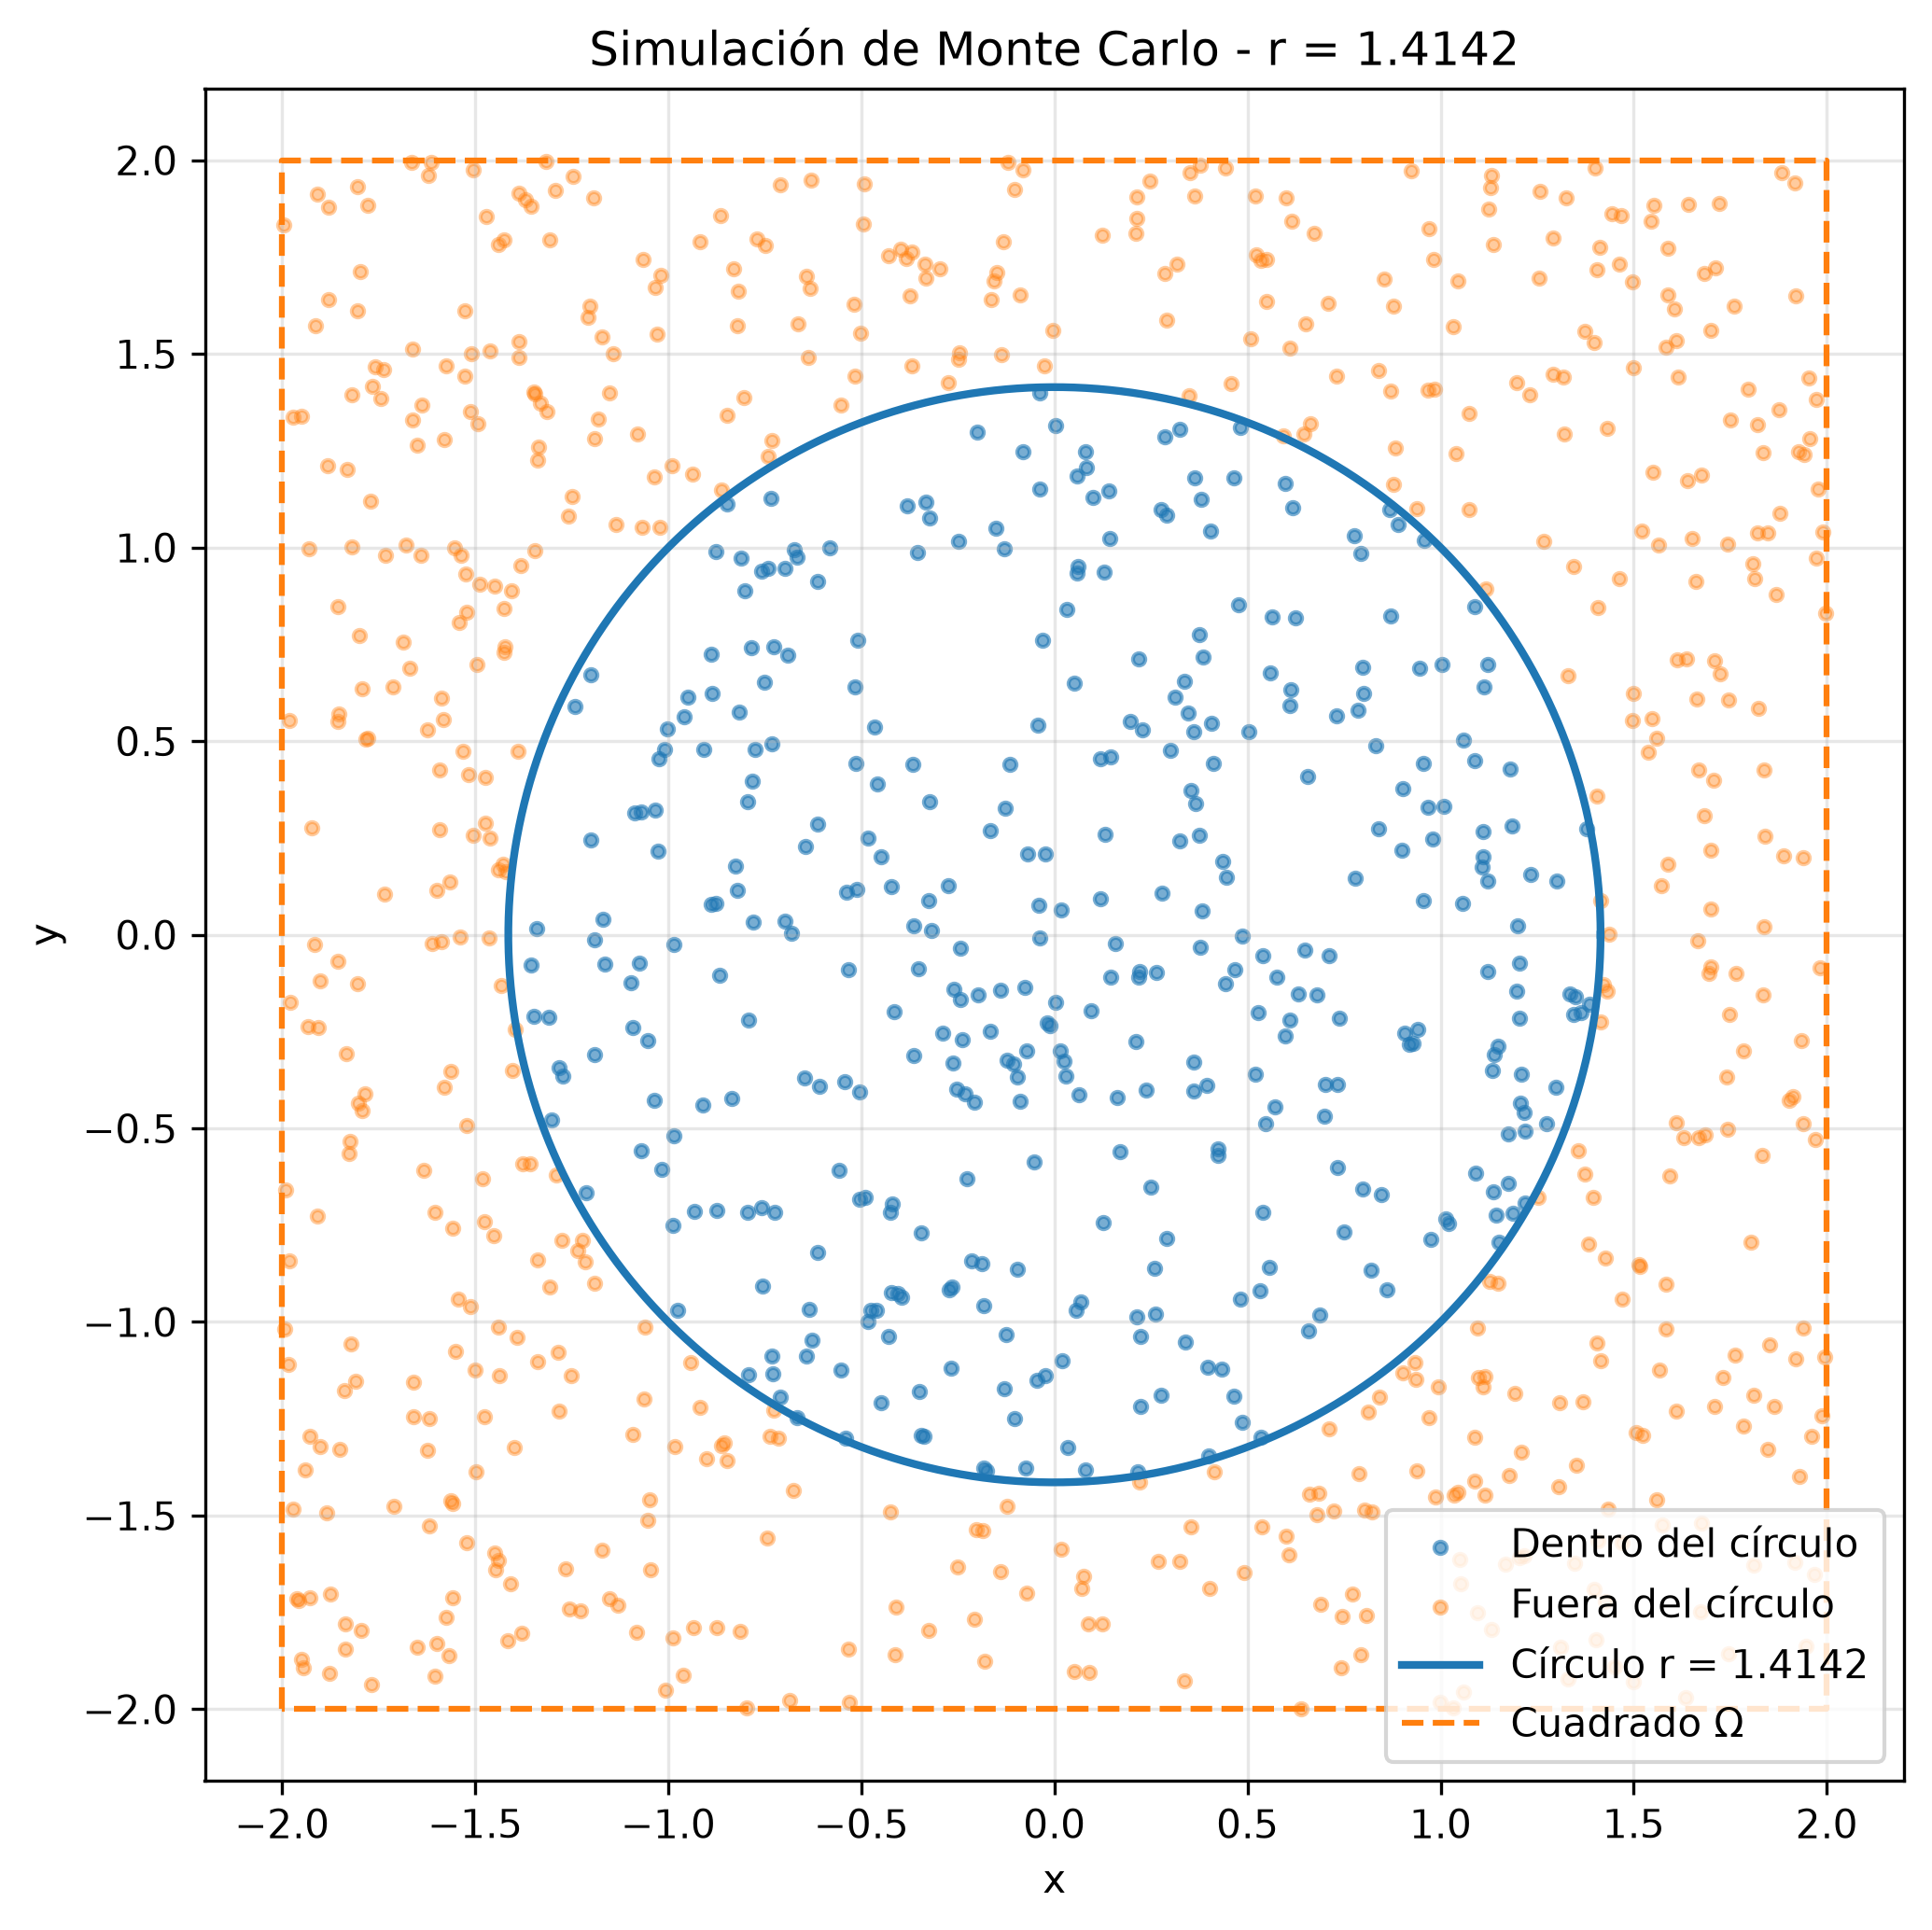
\includegraphics[width=0.75\textwidth]{../results/puntos_radio_1_4142.png}
\caption{Puntos simulados y círculo de radio \(\sqrt{2}\).}
\label{fig:rsqrt2}
\end{figure}

Para \(r=\sqrt{2}\), el círculo ocupa una proporción mayor del dominio
de simulación, permitiendo utilizar una cantidad mayor de puntos en la
estimación.

\subsection{Simulación para \(r=2\)}

\begin{figure}[H]
\centering
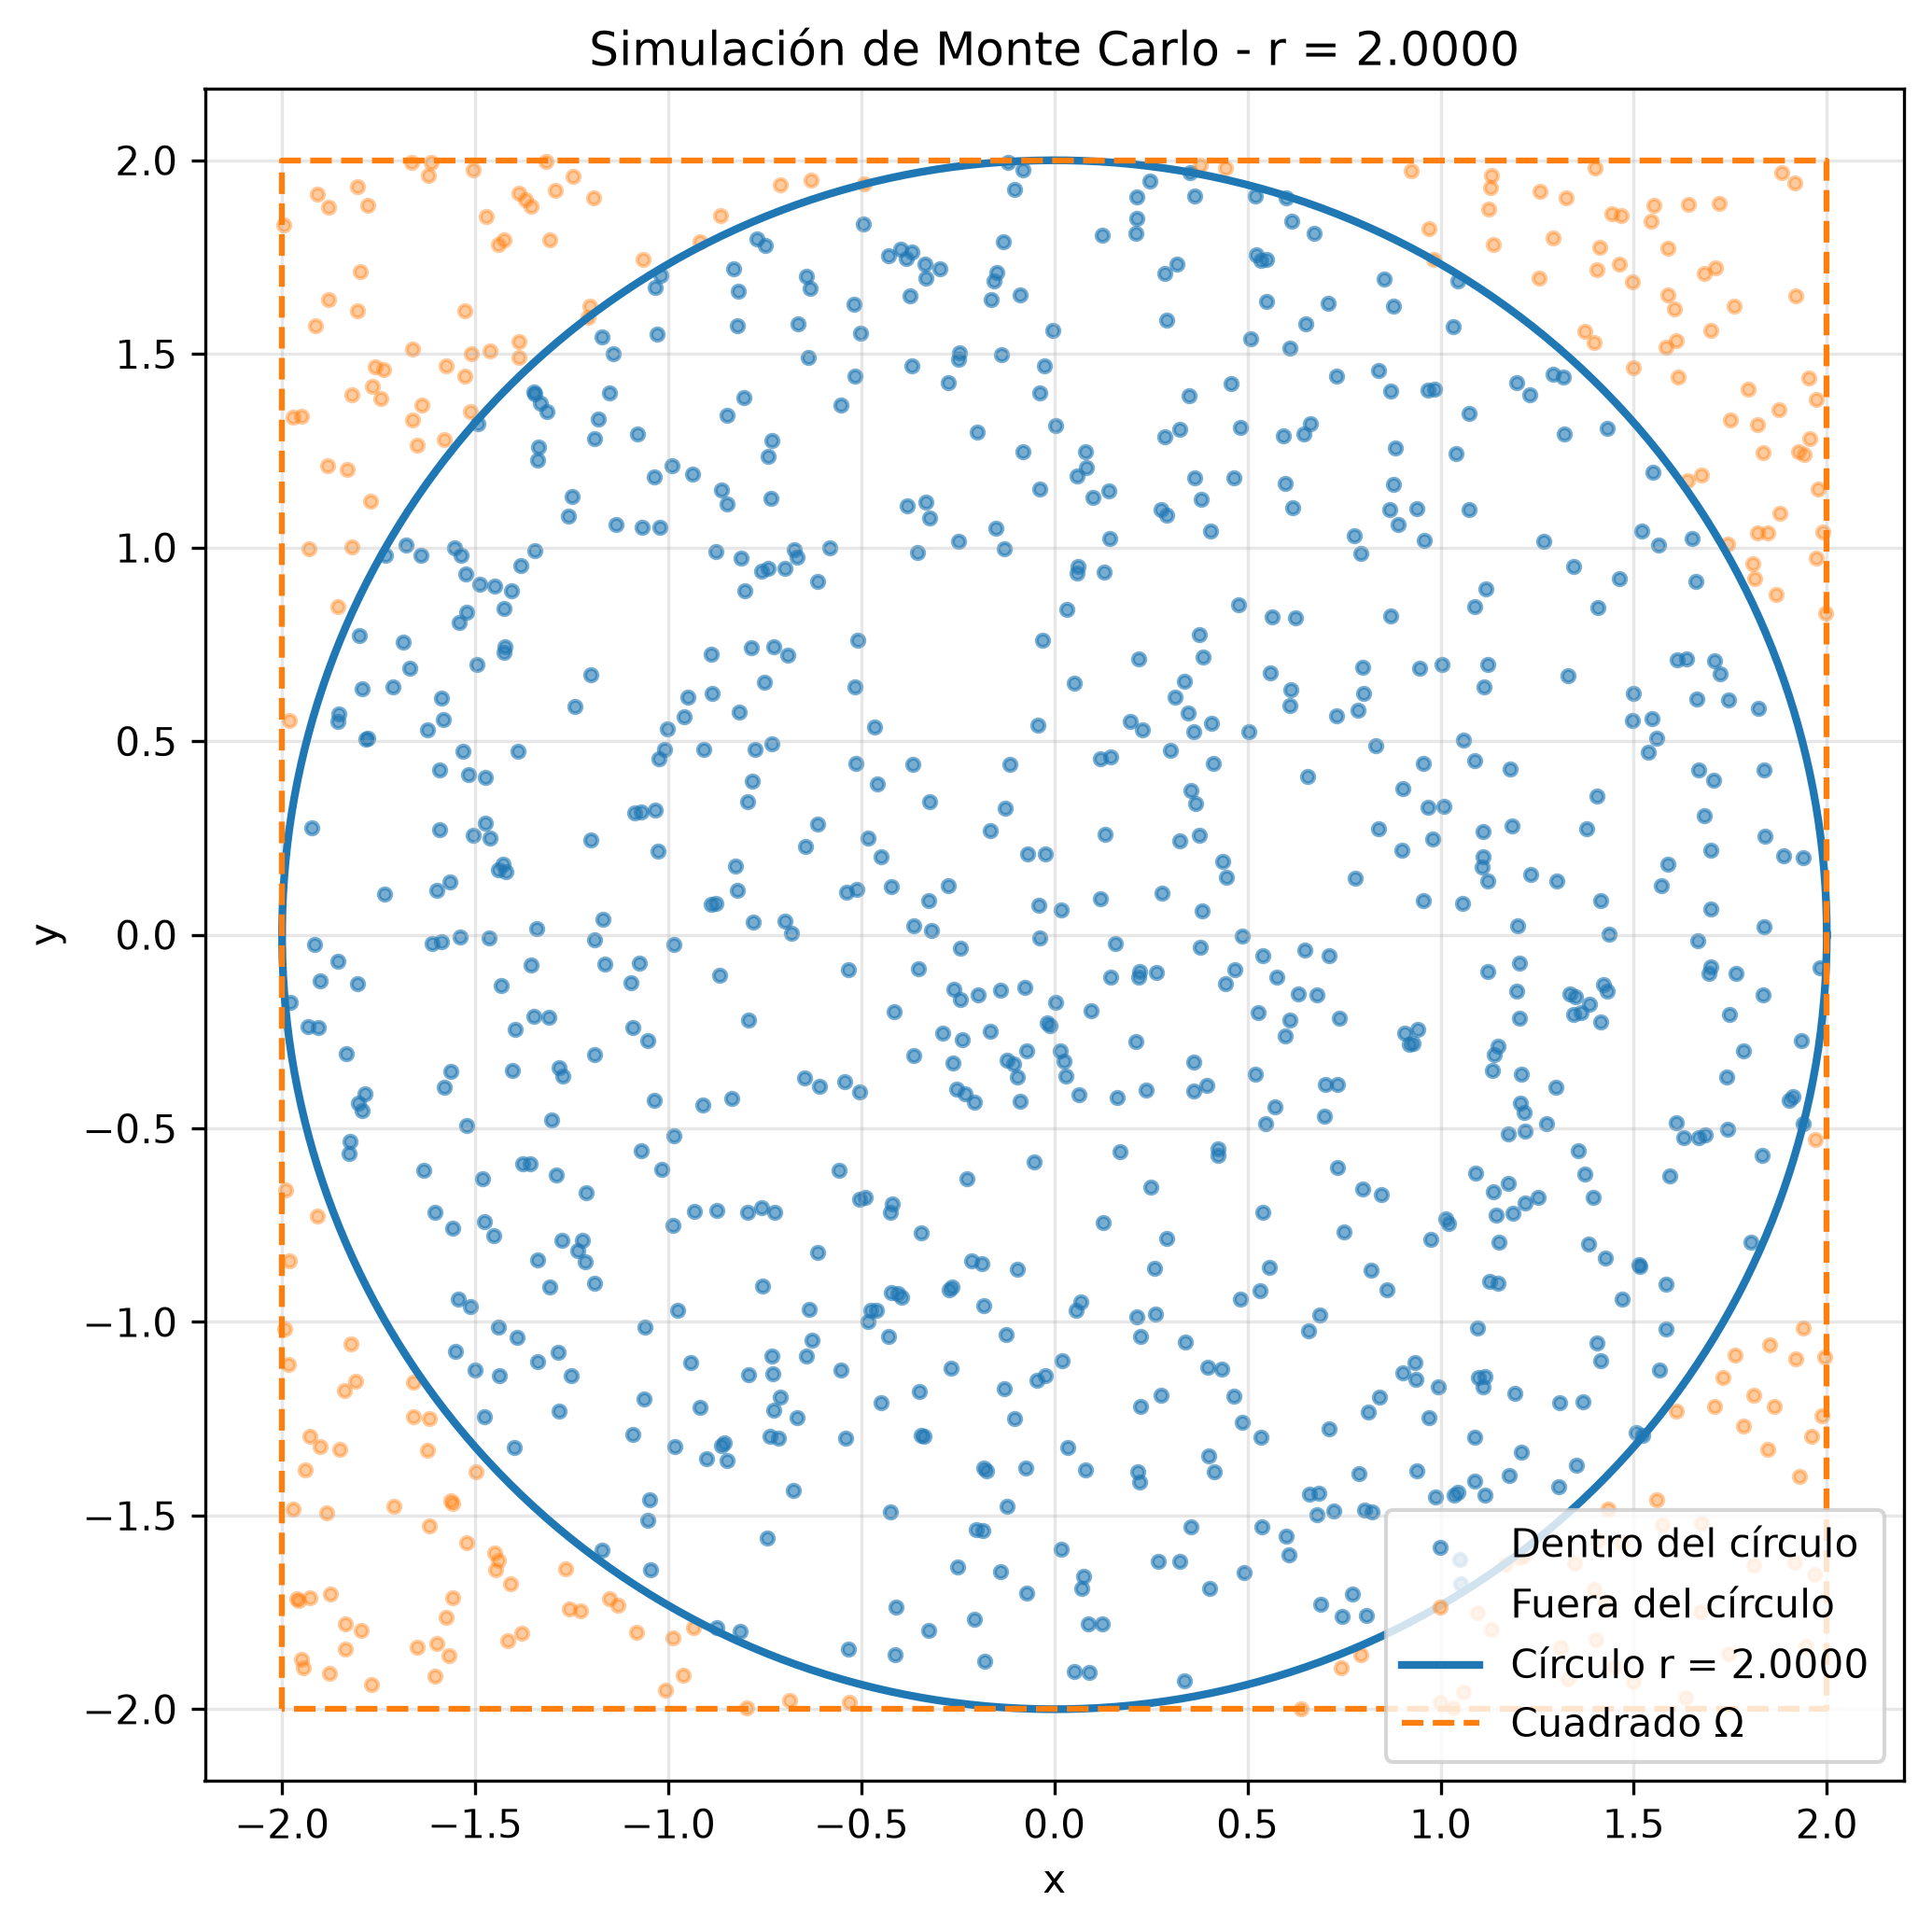
\includegraphics[width=0.75\textwidth]{../results/puntos_radio_2.png}
\caption{Puntos simulados y círculo de radio \(2\).}
\label{fig:r2}
\end{figure}

En este caso el círculo de radio \(2\) se encuentra completamente
contenido en el cuadrado \(\Omega\), alcanzando una mayor proporción
del área total utilizada para la simulación.

% ------------------------------------------------
% 7. ANÁLISIS DE RESULTADOS
% ------------------------------------------------

\section{Análisis de resultados}

\subsection{Comportamiento al aumentar el tamaño de muestra}

Los resultados muestran que el aumento del tamaño de muestra mejora,
en general, la aproximación obtenida mediante Monte Carlo.

Para \(r=1\), por ejemplo, la estimación de \(\pi\) pasa de

\[
4.000000
\]

para \(n=100\) a

\[
3.144272
\]

para \(n=1\,000\,000\).

El error absoluto correspondiente disminuye de

\[
0.858407
\]

a

\[
0.002679.
\]

Sin embargo, el error no disminuye necesariamente de manera monótona.
Por ejemplo, para \(r=1\), el error pasa de

\[
0.029593
\]

para \(n=10\,000\) a

\[
0.031833
\]

para \(n=100\,000\).

Este comportamiento es completamente compatible con el método de
Monte Carlo, puesto que cada estimación depende de una muestra
aleatoria. La Ley de los Grandes Números garantiza convergencia cuando
el tamaño de la muestra crece, pero no exige que cada estimación
sucesiva esté más cerca del valor verdadero.

\subsection{Comparación de los radios}

La comparación entre los radios muestra que las estimaciones obtenidas
con \(r=\sqrt{2}\) y \(r=2\) presentan un comportamiento más estable
que la correspondiente a \(r=1\).

Para \(n=1\,000\,000\), se obtuvieron:

\[
\widehat{\pi}(1)=3.144272,
\]

\[
\widehat{\pi}(\sqrt{2})=3.140752,
\]

\[
\widehat{\pi}(2)=3.142352.
\]

Los errores absolutos son respectivamente

\[
0.002679,\qquad
0.000841,\qquad
0.000759.
\]

Por lo tanto, para el tamaño de muestra más grande utilizado,
\(r=2\) produjo la mejor aproximación.

\subsection{Análisis de la varianza}

Sea

\[
I_r=
\begin{cases}
1, & \text{si el punto pertenece a }C_r,\\
0, & \text{en otro caso}.
\end{cases}
\]

Entonces \(I_r\) es una variable aleatoria de Bernoulli con parámetro

\[
p_r=P(C_r)=\frac{\pi r^2}{16}.
\]

Su varianza es

\[
\operatorname{Var}(I_r)
=
p_r(1-p_r).
\]

Como la estimación de la probabilidad es el promedio de \(n\)
variables indicadoras independientes,

\[
\operatorname{Var}
\left(
\widehat{P}_n(C_r)
\right)
=
\frac{p_r(1-p_r)}{n}.
\]

El estimador de \(\pi\) es

\[
\widehat{\pi}_n(r)
=
\frac{16}{r^2}
\widehat{P}_n(C_r).
\]

Por tanto,

\[
\operatorname{Var}
\left(
\widehat{\pi}_n(r)
\right)
=
\frac{256}{r^4}
\frac{p_r(1-p_r)}{n}.
\]

Sustituyendo

\[
p_r=\frac{\pi r^2}{16},
\]

se obtiene

\[
\operatorname{Var}
\left(
\widehat{\pi}_n(r)
\right)
=
\frac{16\pi}{r^2n}
-
\frac{\pi^2}{n}.
\]

Esta expresión muestra que, para los radios considerados, la varianza
disminuye al aumentar \(r\). En consecuencia, \(r=2\) presenta la
menor varianza teórica entre los tres casos.

Esto es consistente con los resultados obtenidos en la simulación:
para \(n=1\,000\,000\), el radio \(2\) produjo el menor error absoluto.

% ------------------------------------------------
% 8. CONCLUSIONES
% ------------------------------------------------

\section{Conclusiones}

La simulación realizada confirma el comportamiento esperado del método
de Monte Carlo. Al aumentar el número de puntos generados, las
frecuencias relativas utilizadas para aproximar las probabilidades
tienden hacia sus valores teóricos y, consecuentemente, las
estimaciones de \(\pi\) tienden hacia

\[
\pi\approx3.14159265.
\]

Los resultados obtenidos muestran que aumentar el tamaño de muestra
mejora significativamente la precisión de las estimaciones. Para el
círculo unitario, el error absoluto de la aproximación de \(\pi\)
disminuyó desde \(0.858407\) con \(n=100\) hasta \(0.002679\) con
\(n=1\,000\,000\).

Debido a la naturaleza aleatoria del procedimiento, el error no
disminuye necesariamente de manera monótona. Las fluctuaciones
observadas al aumentar \(n\) son consecuencia de la variabilidad
inherente al muestreo aleatorio y no representan un fallo del método.

La comparación entre los tres radios mostró que, para el mayor tamaño
de muestra utilizado, \(r=2\) produjo la mejor aproximación, con un
error absoluto de aproximadamente \(0.000759\). Este comportamiento
también puede justificarse mediante el análisis de la varianza del
estimador, ya que para los radios considerados la varianza disminuye
al aumentar \(r\).

En conclusión, el experimento permite observar de manera práctica la
convergencia asociada a la Ley de los Grandes Números y muestra cómo
un problema geométrico sencillo puede utilizarse para construir un
estimador de una constante matemática fundamental mediante simulación
computacional.

% ------------------------------------------------
% 9. ANEXO
% ------------------------------------------------

\section{Anexo: código utilizado}

El código empleado para realizar las simulaciones se encuentra
organizado en el archivo

\begin{center}
\texttt{src/simulacion.py}
\end{center}


dentro de la estructura del proyecto. El programa genera los puntos
aleatorios, determina la pertenencia a los círculos considerados,
calcula las estimaciones de las probabilidades y de \(\pi\), y genera
las tablas y gráficas utilizadas en este informe.

La separación entre el código fuente, los resultados numéricos y el
informe permite mantener una estructura organizada y reproducible del
proyecto.

\url{https://github.com/Henry2899/cadenas-markov-aplicaciones}

\href{https://github.com/Henry2899/cadenas-markov-aplicaciones/blob/main/tarea-01-monte-carlo/src/simulacion.py}{Ver código fuente}



\end{document}
